\graphicspath{{images/arrangements/}}

\section{Parsimonious representations from 2D partitions}

%\begin{frame}{Approaches}
%	
%\begin{frame}
	
\begin{frame}{Reconstruction pipeline}
	\begin{minipage}[b]{0.2\linewidth}
	\includegraphics[width=\linewidth]{pipeline/pointcloud_crop}
	\end{minipage}%
	\begin{minipage}[b]{0.2\linewidth}
		\includegraphics[width=\linewidth]{pipeline/segments_crop}
	\end{minipage}%
	\begin{minipage}[b]{0.2\linewidth}
		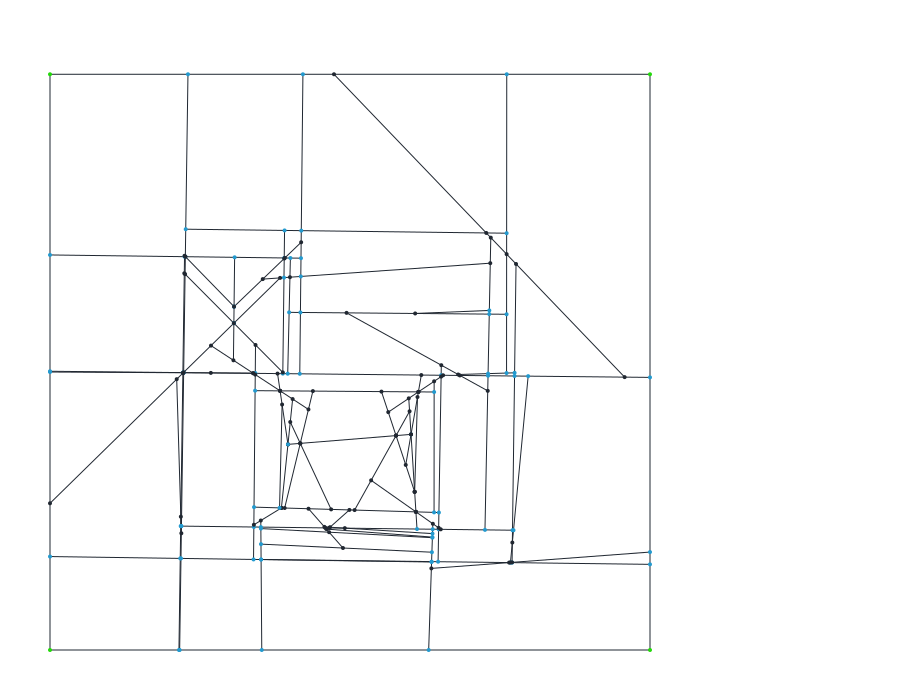
\includegraphics[width=\linewidth]{pipeline/original}
	\end{minipage}%
	\begin{minipage}[b]{0.2\linewidth}
		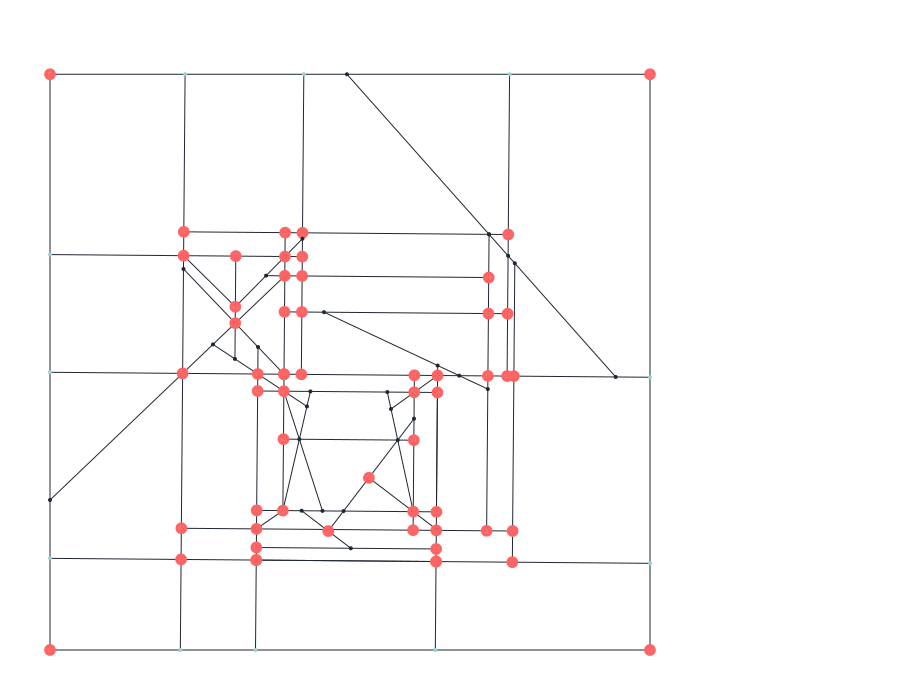
\includegraphics[width=\linewidth]{pipeline/simplified}
	\end{minipage}%
	\begin{minipage}[b]{0.2\linewidth}
		\includegraphics[width=\linewidth]{pipeline/mesh_crop}
	\end{minipage}

	\begin{itemize}
		\item Input: Point clouds, Photogrammetry or Structure-from-Motion (SfM)
		\item Segment detection
		\item Kinetic partition
		\item Simplification
		\item Lifted model (LOD2 representation for GIS)
	\end{itemize}
\end{frame}

\begin{frame}{Segment detection}
	\begin{center}
		\includegraphics[width=0.5\textwidth]{plane_detection}
	\end{center}
	\textbf{Plane detection} using $k$-NN and region-growing \cite{feng_FastPlaneExtraction_2014, holz_FastRangeImage_2013, rabbani_SegmentationPointClouds_2006}.\\
	\textbf{Intersection lines} from adjacent planar primitives.\\
\end{frame}

\begin{frame}{Kinetic cell arrangement}
	
	\textbf{Kinetic cell arrangement} \cite{bauchet_KIPPIKIneticPolygonal_2018}
	\vspace{0.5cm}
	
	\includegraphics[width=\linewidth]{kinetic}

	Many \textbf{collinear segments} in this representation.
\end{frame}

\begin{frame}{Lifted model}
	\scriptsize
	\textbf{MRF formulation}
	\[
		E(\mathcal{L}) = \sum_{\mathcal{C}_i \in \mathcal{C}} E_{\mathcal{C}_i}(\mathcal{L}(\mathcal{C}_i)) + \mu \sum_{e = C_i \cap C_j} V_e(\mathcal{L}(\mathcal{C}_i), \mathcal{L}(\mathcal{C}_j))
	\]
	
	\begin{minipage}{0.6\linewidth}
		\textbf{Fidelity to ``inlier data''}
		\[
			E_{\mathcal{C}_i}(\Pi_k) = \frac{ \mathcal{A}_{\mathcal{C}_i}}{\operatorname{Card}(\mathbf{P}\cap \mathcal{C}_i)} \sum_{p \in \mathbf{P} \cap \mathcal{C}_i} \min(\epsilon, | p_z - \Pi_k(p_x, p_y) |)
		\]
		
		\textbf{Regularity to height jumps}
		\[ V_{e}(\Pi_k, \Pi_l) = p_e \operatorname{length}(e) \operatorname{z_e}(\Pi_k, \Pi_l) \]
	\end{minipage}%
	\begin{minipage}{0.4\linewidth}
		\centering
		\includegraphics[width=\linewidth]{lift_terms}
	\end{minipage}
	\vspace{0.5cm}
	
	Local minima by \textbf{graph-cut optimization} \cite{boykov_FastApproximateEnergy_2001}.
\end{frame}

\begin{frame}{The need for simplification}
	\begin{figure}
		\includegraphics[width=\linewidth]{teaser_v2}
	\end{figure}
	
	\textbf{Complex} 2D partitions\\
	\textbf{Lack regularity} (small segments, angles close to orthogonality)\\
	Collinear segments \textbf{by design}\\
		
	\blfootnote{Dataset from 2015 LiDAR survey of Dublin \cite{laefer_2015AerialLaser_2017}.}
\end{frame}

\begin{frame}{Simplification of 2D partitions}
	\scriptsize
	\textbf{Related point set simplification problems}
	\begin{itemize}
		\item Geometric unit disk cover
		\item Minimum dominating set on unit disk graph
	\end{itemize}
	\textbf{NP-hard} \cite{marathe_SimpleHeuristicsUnit_1995}.
	
	\textbf{Simplification/regularity methods for urban scenes}
	\begin{itemize}
		\item Regularity in input data \cite{zhou_5DDualContouring_2010, monszpart_RAPterRebuildingManmade_2015}
		\item Discrete operations on the partitions \cite{li_ApproximatingShapesImages_2020}
		\item Output mesh simplification \cite{garland_SurfaceSimplificationUsing_1997, salinas_StructureAwareMeshDecimation_2015}
	\end{itemize}

	\textbf{Proposition:} Continuous simplification scheme on 2D partitions.
\end{frame}

\begin{frame}[t]{Point vs. line movement}
	\scriptsize
	
	\begin{minipage}{0.6\linewidth}
		\textbf{Point representation}
		\begin{itemize}
			\item Explicit coordinates for each point.
			\item Lines defined implicitly using two points.
		\end{itemize}	
		\begin{itemize}
			\item[\cmark] Multiple lines can share a same point.
			\item[\xmark] A line cannot carry more than two points.
		\end{itemize}
		
		Preserving collinearities \\
		\hspace{0.05cm} $\implies$ Optimization under constraints.
		
	\end{minipage}%
	\begin{minipage}{0.4\linewidth}
		\includegraphics[width=\linewidth]{point_mouvement}
	\end{minipage}

	\vspace{0.5cm}
	\pause
	
	\textbf{Line representation}
	\begin{itemize}
		\item Explicit coordinates for each line.
		\item Points defined implicitly using two lines.
	\end{itemize}
	\begin{itemize}
		\item[\cmark] A line can carry more than two points.
		\item[\xmark] Multiple lines cannot share a same point.
	\end{itemize}
\end{frame}

\begin{frame}{Optimization on line coordinates}
	\small
	
	\begin{minipage}{0.5\linewidth}
		\textbf{Representation of lines}
		\[ a x + b y + c = 0 \]
	
		\textbf{Euclidean normalization}
		\[ a^2 + b^2 = 1 \]
	\end{minipage}%
	\begin{minipage}{0.5\linewidth}
		\includegraphics[width=\linewidth]{euclidean_normalization_line}
	\end{minipage}
	
	\vspace{1cm}
	
	\textbf{Trade-off between fidelity and regularity}
	\[ 
	E(\mathcal{L}) = E_{fidelity}(\mathcal{L}) + \lambda_1 \: E_{concurrent}(\mathcal{L}) + {\lambda_2} \: E_{orthogonality}(\mathcal{L})
	\]
	
	\blfootnote{Image from \cite{forstner_PhotogrammetricComputerVision_2016}.}
\end{frame}

\begin{frame}[t]{Fidelity term}
	\tiny
	\begin{flalign*}
		&E(\mathcal{L}) = \alert{E_{fidelity}(\mathcal{L})} + \lambda_1 \: E_{concurrent}(\mathcal{L}) + 	{\lambda_2} \: E_{orthogonality}(\mathcal{L})&
	\end{flalign*}
	
	\small
	\textbf{Fidelity term}

	No distance between lines invariant under Euclidean isometries.
	\begin{eqnarray*}
		d(P, L + \delta L)^2 & = & (\delta a \cdot x + \delta b \cdot y + \delta c)^2 \\
		& = &  {\delta L}^t
		\begin{pmatrix}
			x^2 & xy & x \\
			yx & y^2 & y \\
			x & y & 1
		\end{pmatrix} 
		\delta L
	\end{eqnarray*}
	\pause
	\[
		M_i \defunder{=} \frac{1}{2} 
		\begin{bmatrix}
			x_0^2 + x_1^2 + l_{\min}^2 & x_0 y_0 + x_1 y_1 & x_0 + x_1 \\
			x_0 y_0 + x_1 y_1 & y_0^2 + y_1^2  + l_{\min}^2 & y_0 + y_1 \\
			x_0 + x_1  & y_0 + y_1 & 2 
		\end{bmatrix}
	\]
	
	\pause
	\[
		E_{fidelity}(\mathcal{L}) \defunder{=} \frac{1}{2} \sum_{i = 1}^{n} L_i^t M_i L_i
	\]
\end{frame}

\begin{frame}[t]{Regularity terms}
	\tiny
	\begin{flalign*}
		&E(\mathcal{L}) = E_{fidelity}(\mathcal{L}) + \lambda_1 \: \alert{E_{concurrent}(\mathcal{L})} + {\lambda_2} \: \alert{E_{orthogonality}(\mathcal{L})}&
	\end{flalign*}

	\small
	\begin{minipage}{0.7\linewidth}
	\textbf{Line concurrency}
	\begin{eqnarray*}
		D_{ijk} &\defunder{=}& |\det(L_i, L_j, L_k)| \\
		& = & ||P_{ij} - P_{ik}|| \sin \alpha_{ij} \: \sin \alpha_{ik}
	\end{eqnarray*}
	\end{minipage}%
	\begin{minipage}{0.3\linewidth}
		\centering
		\includegraphics[width=\linewidth]{concurrent_config}
	\end{minipage}%
	\[
		E_{concurrent}(\mathcal{L}) = \sum_{(i, j, k) \in \mathcal{T}} \min \left(\epsilon, |\det(L_i, L_j, L_k)| \right)
	\]
	
	\vspace{0.5cm}
	\textbf{Orthogonality}
	\[
		E_{orthogonality}(\mathcal{L}) = \sum_{(i, j) \in \mathcal{P}} \min (\sin \alpha_{\max}, |\operatorname{dot2d}(L_i, L_j) |)
	\]
\end{frame}

\begin{frame}[c]{Riemannian gradient descent (I)}
	\scriptsize
	
	\begin{minipage}[t]{0.5\linewidth}
		\textbf{Euclidean case:} $\nabla f = D^{t}$
	\end{minipage}%
	\pause%
	\begin{minipage}[t]{0.5\linewidth}
		\centering
 		\textbf{Riemannian manifold:} $\nabla f = G^{-1} D^t$
	\end{minipage}%
	
	\begin{center}
	\includegraphics[width=0.5\linewidth]{euclidean_normalization_line}
	\end{center}

	\textbf{Tangent space} of $\mathcal{M}$ at $L_i$:
	\begin{tabular}{cc}
		$ \mathcal{T}_{L_i} \mathcal{M} = \{ v \in \mathbb{R}^3, v \cdot (a,b, 0) = 0 \} = U_i \mathbb{R}^2 $
		& with $U_i = \begin{pmatrix} b & 0 \\ a & 0 \\ 0 & 1 \end{pmatrix}$
	\end{tabular}

	$M_i$, restricted to this $2$-dimensional vector space $\mathcal{T}_{L_i} \mathcal{M}$, is \textbf{non-degenerate}.
%	: it defines a Riemannian metric for the line $L_i$ on $\mathcal{M}$.
\end{frame}

\begin{frame}[c]{Riemannian gradient descent (II)}
	\scriptsize

	\textbf{Derivative} of the objective function
	\[ D_i = \left( \frac{dE }{da},  \frac{dE }{db}, \frac{dE }{dc} \right) \]	
	
	\textbf{Derivative and Riemannian metric} in the tangent space $\mathcal{T}_{L_i} \mathcal{M}$:
	\begin{eqnarray*}
		D_i' &=& D_i U_i \\
		M_i' &=& U_i^t  M_i U_i
	\end{eqnarray*}
	
	\textbf{Gradient} in homogeneous coordinates:
	\[
	\nabla_i E = U_i (M_i')^{-1} {D_i'}^t
	\]
	
	\textbf{Gradient descent} step:
	\[
	\forall i,  \quad L_i^{(k+1)} = normalize\left(  L_i^{(k)} - \alpha \nabla_i E   \right) 
	\]
\end{frame}

\begin{frame}{Combinatorial reductions}
	\scriptsize

	\textbf{Discrete simplification operations}: merging lines.
		
	Two possibilities for $|\det(L_i, L_j, L_k) | = 0$
	\begin{enumerate}
		\item[a.] Two equal lines;
		\item[b.] Lines meets at a same point.
	\end{enumerate}
	
	Special care when using a threshold: $|\det(L_i, L_j, L_k) | < \eta$.
	\pause
	
	\begin{minipage}{0.7\linewidth}
	Merging lines $L_i, L_j$ into $L_f$:
	\[ M_f = M_i + M_j \]
	
	Similar to QEM \cite{garland_SurfaceSimplificationUsing_1997}.
	\end{minipage}%
	\begin{minipage}{0.3\linewidth}
		\centering
		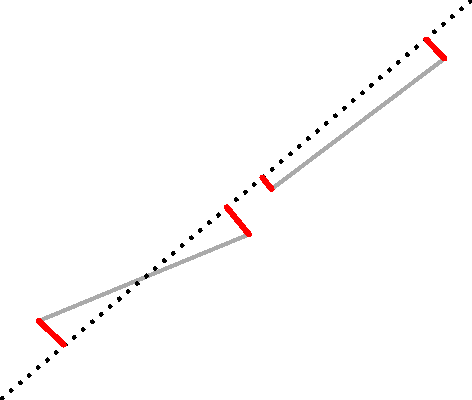
\includegraphics[height=0.6\linewidth]{metric_merge}
	\end{minipage}
\end{frame}

\begin{frame}[c]{Optimization}
	\begin{center}
		\begin{overpic}[width=\textwidth]{arrangement_levels}		
			\put(10,33){\makebox[0pt]{\fontsize{6}{6}\textsc{Iteration 0}}}
			\put(10,31){\makebox[0pt]{\fontsize{6}{6}\selectfont{Complexity: 1,121}}}
			\put(10,29){\makebox[0pt]{\fontsize{6}{6}\selectfont{Orthogonality: 0}}}
			
			\put(30,33){\makebox[0pt]{\fontsize{6}{6}\textsc{Iteration 1000}}}
			\put(30,31){\makebox[0pt]{\fontsize{6}{6}\selectfont{Complexity: 812}}}
			\put(30,29){\makebox[0pt]{\fontsize{6}{6}\selectfont{Orthogonality: 529}}}
			
			\put(50,33){\makebox[0pt]{\fontsize{6}{6}\textsc{Iteration 3000}}}
			\put(50,31){\makebox[0pt]{\fontsize{6}{6}\selectfont{Complexity: 518}}}
			\put(50,29){\makebox[0pt]{\fontsize{6}{6}\selectfont{Orthogonality: 391}}}
			
			\put(70,33){\makebox[0pt]{\fontsize{6}{6}\textsc{Iteration 7000}}}
			\put(70,31){\makebox[0pt]{\fontsize{6}{6}\selectfont{Complexity: 137}}}
			\put(70,29){\makebox[0pt]{\fontsize{6}{6}\selectfont{Orthogonality: 161}}}
			
			\put(90,33){\makebox[0pt]{\fontsize{6}{6}\textsc{Iteration 9000}}}
			\put(90,31){\makebox[0pt]{\fontsize{6}{6}\selectfont{Complexity: 44}}}
			\put(90,29){\makebox[0pt]{\fontsize{6}{6}\selectfont{Orthogonality: 57}}}
		\end{overpic}
	\end{center}
\end{frame}

\begin{frame}{Comparison}
	\centering
	\tiny
	\begin{overpic}[width=0.9\linewidth]{comparisons_v2}
		%Laser
		\put(0,30){\fontsize{7}{7}\selectfont{LiDAR}}
		
		\put(30,56.5){\fontsize{7}{7}\selectfont{QEM}}
		\put(45,46.5){\fontsize{5}{5}\selectfont{error: 0.079}}
		\put(45,45.5){\fontsize{5}{5}\selectfont{complexity: 15}}
		
		\put(30,42.5){\fontsize{7}{7}\selectfont{SAMD}}
		\put(45,33.5){\fontsize{5}{5}\selectfont{error: 0.085}}
		\put(45,32.5){\fontsize{5}{5}\selectfont{complexity: 16}}
		
		\put(54,56.5){\fontsize{7}{7}\selectfont{RPP}}
		\put(69,46.5){\fontsize{5}{5}\selectfont{error: 0.032}}
		\put(69,45.5){\fontsize{5}{5}\selectfont{complexity: 814}}
		
		\put(54,42.5){\fontsize{7}{7}\selectfont{VSA}}
		\put(69,33.5){\fontsize{5}{5}\selectfont{error: 0.072}}
		\put(69,32.5){\fontsize{5}{5}\selectfont{complexity: 501}}
		
		\put(76,56.5){\fontsize{7}{7}\selectfont{Ours (w/o simpl.)}}
		\put(93,46.5){\fontsize{5}{5}\selectfont{error: 0.074}}
		\put(93,45.5){\fontsize{5}{5}\selectfont{complexity: 33}}
		
		\put(76,42.5){\fontsize{7}{7}\selectfont{Ours}}
		\put(93,33.5){\fontsize{5}{5}\selectfont{error: 0.054}}
		\put(93,32.5){\fontsize{5}{5}\selectfont{complexity: 15}}
		
		%MVS
		\put(0,25){\fontsize{7}{7}\selectfont{Photogrammetry}}
		
		\put(30,25){\fontsize{7}{7}\selectfont{QEM}}
		\put(45,16){\fontsize{5}{5}\selectfont{error: 0.097}}
		\put(45,15){\fontsize{5}{5}\selectfont{complexity: 24}}
		
		\put(30,12.5){\fontsize{7}{7}\selectfont{SAMD}}
		\put(45,3){\fontsize{5}{5}\selectfont{error: 0.07}}
		\put(45,2){\fontsize{5}{5}\selectfont{complexity: 25}}
		
		\put(54,25){\fontsize{7}{7}\selectfont{RPP}}
		\put(69,16){\fontsize{5}{5}\selectfont{error: 0.044}}
		\put(69,15){\fontsize{5}{5}\selectfont{complexity: 28}}
		
		\put(54,12.5){\fontsize{7}{7}\selectfont{VSA}}
		\put(69,3){\fontsize{5}{5}\selectfont{error: 0.03}}
		\put(69,2){\fontsize{5}{5}\selectfont{complexity: 717}}
		
		\put(76,25){\fontsize{7}{7}\selectfont{Ours (w/o simpl.)}}
		\put(93,16){\fontsize{5}{5}\selectfont{error: 0.07}}
		\put(93,15){\fontsize{5}{5}\selectfont{complexity: 186}}
		
		\put(76,12.5){\fontsize{7}{7}\selectfont{Ours}}
		\put(93,3){\fontsize{5}{5}\selectfont{error: 0.055}}
		\put(93,2){\fontsize{5}{5}\selectfont{complexity: 24}}
	\end{overpic}
\end{frame}

\begin{frame}[c]{Results}
	\includegraphics[width=0.5\linewidth]{bb_v2}%
	\includegraphics[width=0.5\linewidth]{hoteldieu_v3}
\end{frame}

\begin{frame}{Limitations}
	\small
	\textbf{Representability} of the LOD2 model
	\begin{center}
		\includegraphics[width=0.6\linewidth]{failure_case}
	\end{center}

	\textbf{Dissociation} between 2D and 3D regularity
	\begin{center}
		\includegraphics[width=0.8\linewidth]{closeup_v2}
	\end{center}
\end{frame}
